\documentclass[11pt,letterpaper]{amsart}
\usepackage[letterpaper,textwidth=31pc,textheight=50\baselineskip,marginparwidth=1.15in,marginparsep=1.4em,centering,includehead]{geometry}
\usepackage{iftex,etoolbox}
\usepackage{amsmath,amssymb,amsthm,booktabs,float}
\ifPDFTeX
 \usepackage[T1]{fontenc}
 \usepackage{newpxtext}
 \usepackage[euler-digits,euler-hat-accent]{eulervm}
 \usepackage[final,tracking=smallcaps,expansion=true,protrusion=true]{microtype}
\else
 \usepackage[no-math]{fontspec}
 \setmainfont{texgyrepagella}[Extension=.otf,UprightFont=*-regular,BoldFont=*-bold,ItalicFont=*-italic,BoldItalicFont=*-bolditalic]
 \usepackage[euler-digits,euler-hat-accent]{eulervm}
 \DeclareSymbolFont{operators}{OT1}{pplx}{m}{n}
 \SetSymbolFont{operators}{bold}{OT1}{pplx}{b}{n}
 \usepackage[final,protrusion=true]{microtype}
\fi
\usepackage[authoryear,round]{natbib}
\usepackage{graphicx,url,xcolor}
\urlstyle{same}
\makeatletter\g@addto@macro\UrlBreaks{\do\_}\makeatother
\newcommand{\leanname}[1]{{\urlstyle{tt}\nolinkurl{#1}}}
\usepackage{hyperref}
\definecolor{linkink}{rgb}{0.12,0.22,0.48}
\hypersetup{colorlinks,linkcolor=linkink,citecolor=linkink,urlcolor=linkink,
 pdftitle={A Needle in Five Tiny Haystacks: Local Learning Coefficients of Scalar ResNets},
 pdfauthor={Bobby Faber}, pdfsubject={Local learning coefficients of scalar polynomial residual networks},
 pdfkeywords={singular learning theory, residual networks, real log canonical threshold, Lean}}
\clubpenalty=10000
\widowpenalty=10000
\displaywidowpenalty=10000
\linespread{1.04}
\setlength{\emergencystretch}{2.5em}
\newtheoremstyle{scplain}{.7\baselineskip}{.7\baselineskip}{\itshape}{}{\bfseries\scshape}{.}{.5em}{}
\theoremstyle{scplain}
\newtheorem{theorem}{Theorem}
\newtheorem{lemma}{Lemma}[section]
\newcommand{\R}{{\mathbb R}}
\newcommand{\asym}{\asymp}
\newcommand{\norm}[1]{\left\lVert#1\right\rVert}
\newcommand{\pos}[1]{(#1)_+}
\DeclareMathOperator{\supp}{supp}
\makeatletter
\patchcmd{\@maketitle}{\global\topskip42\p@}{\global\topskip6\p@}{}{\PackageWarning{style}{title patch failed}}
\renewcommand\paragraph{\@startsection{paragraph}{4}{\z@}{.6\baselineskip\@plus.2\baselineskip}{-.6em}{\normalfont\scshape}}
\makeatother

% Marginal Lean tag linking to the certifying declaration at the pinned snapshot.
\newcommand{\leantag}[2]{\marginpar{\raggedright\footnotesize\textsc{lean}~\href{https://github.com/bubskee/residual-slt-in-a-haystack/blob/b08b1a334abac97cbdf754ba14eacee82e10be70/lean/ResidualSLT/#1.lean\#L#2}{\checkmark}\\[-1pt]{\fontsize{6.5}{8}\selectfont\itshape\hspace{0pt}#1}}}
\title[A Needle in Five Tiny Haystacks]{A Needle in Five Tiny Haystacks:\\Local Learning Coefficients of Scalar ResNets}
\author{Bobby Faber}
\address{Independent}
\date{7 November 2026}
\subjclass[2020]{62F15; 14E15, 68T07}
\keywords{singular learning theory, residual networks, real log canonical threshold, Newton polyhedra, Lean}
\begin{document}
\begin{abstract}
The same function can have different local learning coefficients at different realizations of a residual network. We determine the local learning coefficient $\lambda$ and multiplicity $m$ on the degenerate locus of the scalar polynomial residual networks of Dahlgren, Marchetti and Kohn: compositions of $L$ blocks $x\mapsto x+w^rx^r$, with squared-error loss and priors in the raw weights $w$. Already at depth five, the cubic target $f(x)=x+x^3$ has five realizations with a single nonzero weight but three local pairs, $(13/12,1)$, $(7/6,2)$ and $(7/6,1)$. The difference is decided by the lengths of the consecutive inactive groups between and around the nonzero blocks. For odd $r$, signed powers can cancel within a group; this lowers the exponent once the group is longer than $r$ and produces a logarithm at length exactly $r$. We compute the local pair for every degree, depth and arrangement of active blocks, classify and count the complete target fibers, and determine the globally dominant pair. Lean~4 certifies the pairs, fibers and counts of all three theorems for localizations on small balls with bounded measurable densities, under the stated Gram assumption.
\end{abstract}
\maketitle

\section{Introduction}
A depth-five cubic residual network computes $f(x)=x+x^3$ when exactly one of its five raw weights is one and the others are zero. These five parameter vectors give the same function, but their local loss integrals differ. Write $(\lambda,m)$ for the local learning coefficient and multiplicity, so that the integral of $e^{-NK_f}$ near a realization has order $N^{-\lambda}(\log N)^{m-1}$ as the concentration parameter $N\to\infty$, where $K_f$ is the squared-error population loss. At the two endpoints the pair is $(13/12,1)$; one position inward it is $(7/6,2)$; at the center it is $(7/6,1)$ (Figure~\ref{fig:arrangements}, Table~\ref{tab:examples}). The needle in the title is the one active block. What changes from one realization to the next is how the four inactive blocks are grouped around it, and that grouping alone decides the pair.

The question comes from \citet{dahlgren2026}. They prove that polynomial residual networks are generically identifiable: for a generic parameter, the parameters computing the same function are determined up to explicit symmetries. Their results apply to nondegenerate parameters, those at which no neuron is the zero polynomial. For the rest they write that ``a classification of fibers on the degenerate locus remains open'': such a fiber may be a further discrete orbit or may contain positive-dimensional families, and the effect of these singularities on training and generalization is unknown. In width one a neuron is a single weight times the incoming state, so a dead neuron is a zero weight, and a block with zero weight is the identity map. The degenerate locus is exactly the set of realizations with inactive blocks, and the five realizations above are its smallest nontrivial instance. We started by computing their pairs and then carried the computation through every degree $r\ge2$, depth $L\ge1$ and number of active blocks. Every target fiber is finite: its points are the placements of the ordered active blocks, with sign choices when $r$ is even, and Theorem~\ref{thm:global} counts them. Theorem~\ref{thm:arrangement} gives the pair at each point from the identity-target calculation of Theorem~\ref{thm:identity}, and in singular learning theory that pair measures the effect of the singularity on Bayesian learning \citep{watanabe2009}. Lean~4 certifies all three theorems.

The example separates properties of a represented function from properties of its realizations. The local learning coefficient belongs to a point in parameter space \citep{watanabe2009,lau2025}, and neither parameter count nor Jacobian rank determines it \citep{wei2023}. All five realizations have five raw parameters and coefficient-Jacobian rank one, yet their pairs differ. The distinction matters when $\lambda$ is estimated around a trained solution: the estimate describes the neighborhood reached, not every parameter vector computing the same function. Here different neighborhoods can have exponents separated by $1/12$, and equal exponents can carry different logarithmic multiplicities; the remark in Section~5 spells out what an averaged quantity detects. At the global level the realizations with the smallest $\lambda$ carry the integral. At depth five these are the endpoints, where all four inactive weights form one group: one long group is cheaper than two short ones, because more weights can cancel together. Theorem~\ref{thm:global} determines the dominant pair at every depth and active count.

The reason position matters is cancellation. Moving the active block along a chain of identity blocks does not change the output. Perturbing consecutive inactive weights does change it, and for odd $r$ the leading terms are signed $r$th powers that can cancel within the group. An active block between two groups composes their contributions with a nonlinear map, which places them in independent leading coefficient directions (Appendix~\ref{app:arrangement}), so cancellation never crosses an active block. The lengths of the inactive groups, not only the number of zero weights, decide the singular contribution. Theorem~\ref{thm:identity} computes the contribution of one group, and Theorem~\ref{thm:arrangement} adds those contributions to the regular contribution of the active weights. When a group has length exactly $r$, two scaling regimes meet and produce a logarithm.

The architecture is the scalar monomial specialization of the polynomial ResNets of \citet{dahlgren2026}. \citet{shahverdi2026} connect sparse subnetworks with singularities of polynomial function spaces, and \citet{kohn2026} relate rank-deficient critical points of deep monomial networks to subnetworks with inactive neurons; our realizations are subnetworks of exactly this kind, and they show concretely why equal Jacobian rank need not give an equal learning coefficient. Exact coefficients are also known for reduced-rank regression and multilayer linear networks \citep{aoyagiwatanabe2005,aoyagi2024}. We use the singular learning framework of \citet{watanabe2009} and the monomial integration rules of \citet{lin2017}, and the exact values here are test cases for local learning coefficient estimation \citep{lau2025}.

The restriction to scalar, bias-free, monomial blocks is deliberate. It makes every fiber classifiable and every local and global pair computable and certifiable rather than estimated; it is not a model of practical networks. Within it, the theorems give exact local and global pairs for every degree, depth and active count, show that the learning coefficient depends on the realization and not only on the function, explain the dependence by cancellation within inactive groups, and place the odd-degree transition exactly where Newton nondegeneracy fails (Section~3). All statements concern deterministic population-loss integrals with priors in raw weights. Finite samples, training dynamics, stochastic estimators such as that of \citet{lau2025}, and networks with width or biases are outside their scope.

\section{Model and assumptions}\label{sec:model}
Fix integers $r\ge2$ and $L\ge1$. The parameters are the raw block weights $w=(w_1,\ldots,w_L)\in\R^L$, with
\begin{equation}\label{eq:network}
 h_0(x)=x,\qquad h_\ell(x)=h_{\ell-1}(x)+w_\ell^r h_{\ell-1}(x)^r,
 \quad 1\le\ell\le L.
\end{equation}
This is the bias-free scalar specialization of $h\mapsto h+\sigma(wh)$ with $\sigma(z)=z^r$ \citep[Definition 2.1]{dahlgren2026}, hence the coefficient $w^r$. The weights are raw: priors are densities in $w$, not in $c=w^r$. This choice changes the answer, because $w\mapsto w^r$ is not a local diffeomorphism at zero, and a smooth prior in $c$ corresponds to a raw density proportional to $|w|^{r-1}$, which vanishes there. Write $F_c(x)=x+cx^r$, so $h_L=F_{w_L^r}\circ\cdots\circ F_{w_1^r}$. The target $f$ is realizable in this architecture. For an input probability measure $\mu$, let
\begin{equation}\label{eq:loss}
 K_f(w)=\int_\R (h_L(w,x)-f(x))^2\,d\mu(x).
\end{equation}
Put $\nu=(r^L-1)/(r-1)$ and $d_j=1+j(r-1)$ for $1\le j\le\nu$. Throughout, assume the sparse feature Gram matrix
\begin{equation}\label{eq:gram}
 G_{ij}=\int_\R x^{d_i+d_j}\,d\mu(x)
 \quad(1\le i,j\le\nu)
 \quad\text{is finite and positive definite.}
\end{equation}
Then $K_f$ is comparable to the squared coefficient-error norm. A finite absolute moment of order $2r^L$ and infinite support of $\mu$ suffice: a nonzero univariate polynomial has finitely many zeros.

At a realization $w^*$, let $\pi$ be a smooth positive density on a full neighborhood. Take a nonnegative smooth compact cutoff $\chi$, supported in a sufficiently small neighborhood and equal to one near $w^*$. Define the local pair by
\begin{equation}\label{eq:pair}
 Z_{N,w^*}=\int_{\R^L}\chi(w)e^{-N K_f(w)}\pi(w)\,dw
 \asym N^{-\lambda}(\log N)^{m-1},\qquad N\longrightarrow\infty.
\end{equation}
The symbol $\asym$ denotes bounds by positive constant multiples. Equivalently, the local volume of $\{K_f\le\epsilon\}$ has order $\epsilon^\lambda(\log(1/\epsilon))^{m-1}$ as $\epsilon\downarrow0$. A measurable density bounded above and away from zero already suffices for this order; local constants may depend on $r$, $L$, $w^*$ and $\mu$. Appendix~\ref{app:sectors} shows directly, without resolution of singularities, that $\lambda$ is also the local integrability threshold of $K_f^{-s}$ for every loss treated below. For this analytic loss, $m$ is the order of the first positive pole of the local zeta integral, by the usual resolution framework \citep[Theorem 2.10 and Proposition 3.2]{lin2017}; we use this only as an interpretation.\footnote{Because our loss is squared, Lin's coefficient-ideal threshold is $2\lambda$; his zeta convention is $(\sum_i f_i^2)^{-z/2}$.} Global statements use a nonnegative measurable density on $\R^L$ with finite mass, continuous and strictly positive at every point of the target fiber.

\section{The identity-target phase transition}
Write $K_0=K_x$ and $u_i=w_i^r$, and set
\[
 S(w)=\sum_{i=1}^L w_i^r,\qquad Q(w)=\sum_{i=1}^L w_i^{2r}.
\]
\begin{theorem}[Identity target]\label{thm:identity}\leantag{SparseIdentityCertificate}{16}
Under \eqref{eq:gram}, near $w=0$,
\begin{equation}\label{eq:identityreduction}
 K_0(w)\asym S(w)^2+Q(w)^2.
\end{equation}
The local pair is
\begin{equation}\label{eq:identitypair}
 (\lambda,m)=
 \begin{cases}
 (L/(2r),1),&r\text{ even or }L<r,\\
 (1/2,2),&r\text{ odd},\ L=r,\\
 ((L+r)/(4r),1),&r\text{ odd},\ L>r.
 \end{cases}
\end{equation}
Moreover, $K_0$ is coercive and has zero set $\{0\}$. Thus the same pair governs the global integral under a finite-mass prior continuous and positive at zero.
\end{theorem}

\paragraph{What is classical.}
For even $r$ the pair follows from radial scaling (see below). For odd $r$, compare the full loss with its leading term: $S^2$ alone has pair $\bigl(\min\{1/2,L/(2r)\},m\bigr)$ with $m=2$ exactly when $L=r$: $S$ is homogeneous with zero set smooth away from the origin, and the blow-up of Appendix~\ref{app:sectors} without the $Q^2$ term gives a transverse exponent $1/2$ and a radial exponent $L/(2r)$. Thus the leading-term threshold is correct through $L=r$, including the logarithm at equality. For $L>r$ the radial term $Q^2$ cuts off the cancellation cone $\{S=0\}$ and raises $\lambda$ from $1/2$ to $(L+r)/(4r)$. With a smooth positive prior in effective coordinates $u=w^r$, the loss is comparable to $(\sum_iu_i)^2+\norm{u}^4$, whose pair is $(1/2+(L-1)/4,1)$ for every $r$ and $L$. The parity split, the critical length and the logarithm all come from the raw parametrization.

The first two output error coefficients are exactly $S$ and
\[
 B=r\sum_{i<j}u_i u_j=\frac r2(S^2-Q).
\]
All higher coefficients have higher homogeneous degree in $u$. The Gram bound and this identity give \eqref{eq:identityreduction}; Appendix~\ref{app:coeff} supplies the uniform estimate and coercivity argument.

For even $r$, the summands of $S$ are nonnegative, so $S^2\asym\norm{w}^{2r}$ and the radial exponent is $L/(2r)$. For odd $r$ and $L\ge2$, write $w=\rho\theta$ with $\theta\in\mathbb S^{L-1}$. The angular function $\tau(\theta)=\sum_i\theta_i^r$ has a nonempty regular zero set. Near it, transverse coordinates $t=\tau(\theta)$ reduce the loss and volume to
\begin{equation}\label{eq:angularmodel}
 \rho^{2r}(t^2+\rho^{2r}),\qquad
 \rho^{L-1}\,d\rho\,dt\,d\eta
\end{equation}
up to bounded positive factors. A finite collection of local charts with bounded positive densities suffices. In the thin region $|t|\le\rho^r$, cancellation changes the radial scale to $\rho^{4r}$ while the angular width contributes $\rho^r$. This gives \mbox{$(L+r)/(4r)$}. The competing exponent is $L/(2r)$; their crossing at $L=r$ produces one logarithm. Appendix~\ref{app:sectors} computes both exponents and the logarithm using two explicit sectors.

\paragraph{Remark (Newton polyhedra).}
The degree-$2r$ part of $K_0$ is $G_{11}S^2$ and all other terms have higher degree, so the Newton polyhedron of $K_0$ at zero is $\{\alpha\in\R^L_{\ge0}:\sum_i\alpha_i\ge2r\}$ and its Newton prediction \citep{varchenko1976,agzv1988} is $(L/(2r),1)$. The prediction is always an upper bound for $\lambda$, since $S^2\le LQ$ gives $K_0\le C\sum_iw_i^{2r}$. For even $r$, or $L=1$, the face polynomial $G_{11}S^2$ has no zeros in $(\R^*)^L$, in particular no singular ones, and the prediction is exact. For odd $r$ and $L\ge2$ it vanishes to second order on $\{S=0\}\cap(\R^*)^L$, which contains \mbox{$(1,\ldots,1,-(L-1)^{1/r})$}, so $K_0$ is Newton-degenerate. The degeneracy is invisible for $L<r$, where the cancellation exponent $(L+r)/(4r)$ exceeds $L/(2r)$; it costs the logarithm at $L=r$, and lowers $\lambda$ to \mbox{$(L+r)/(4r)$} for $L>r$.

\section{The local arrangement theorem}
Theorem~\ref{thm:identity} supplies the contribution of each consecutive inactive group; the active weights contribute regular directions. For an inactive group of size $n$, define $A_r(0)=0$, $M_r(0)=1$, and, for $n\ge1$,
\begin{equation}\label{eq:AM}
\begin{gathered}
 A_r(n)=\begin{cases}n/(2r),&r\text{ even},\\
 n/(2r)-\pos{n-r}/(4r),&r\text{ odd},\end{cases}
 \\[2pt]
 M_r(n)=\begin{cases}2,&r\text{ odd and }n=r,\\1,&\text{otherwise}.\end{cases}
\end{gathered}
\end{equation}
Here $(a)_+=\max(a,0)$. These are the identity pairs of Theorem~\ref{thm:identity}, with the empty group contributing an integral equal to one.

Fix $w^*$ with exactly $k$ nonzero weights, at positions $i_1<\cdots<i_k$. Put $c_j=(w^*_{i_j})^r\ne0$. There are $k+1$ consecutive inactive groups, of lengths $n_0,\ldots,n_k$, before, between, and after the active blocks; $k+\sum_g n_g=L$. Write their raw weights as $a_g=(a_{g,1},\ldots,a_{g,n_g})$ and put
\[
 S_g=\sum_{i=1}^{n_g}a_{g,i}^r,\qquad Q_g=\sum_{i=1}^{n_g}a_{g,i}^{2r}.
\]
The active deviations $\delta_j=w_{i_j}^r-c_j$ are valid local coordinates because $r(w^*_{i_j})^{r-1}\ne0$.

\begin{samepage}
\begin{theorem}[Local arrangement]\label{thm:arrangement}\leantag{ArrangementCertificate}{31}
Let $f=h_L(w^*,\cdot)$ and assume \eqref{eq:gram}, with any nonzero active values and any inactive group sizes $n_g\ge0$. For odd $r\ge3$, on a sufficiently small full neighborhood of $w^*$,
\begin{equation}\label{eq:arrangementodd}
 K_f\asym\sum_{j=1}^k\delta_j^2+\sum_{g=0}^k(S_g^2+Q_g^2).
\end{equation}
For even $r\ge2$ the comparison is
\begin{equation}\label{eq:arrangementeven}
 K_f\asym\sum_{j=1}^k\delta_j^2+\sum_{\text{inactive }i}|w_i|^{2r}.
\end{equation}
Under the local prior conditions of Section~\ref{sec:model}, for every $k\ge0$ with total depth $L\ge1$,
\begin{equation}\label{eq:arrangementpair}
 \boxed{\lambda=\frac{k}{2}+\sum_{g=0}^k A_r(n_g),\qquad
 m=1+\sum_{g=0}^k\bigl(M_r(n_g)-1\bigr).}
\end{equation}
\end{theorem}
\end{samepage}

Independence of the retained directions follows by induction on active count: each new active block multiplies old directions by a polynomial coprime to the new active direction, while the new group directions have strictly higher degree.

Independence controls the retained coefficient directions, but cancellations can make those coefficients much smaller than the raw perturbation. A remainder estimate solely in the raw distance would then be insufficient: the omitted terms must be small relative to the retained coefficients themselves. Appendix~\ref{app:arrangement} proves $\norm{E}\le C\varepsilon\norm{z}$, where $z$ collects the retained active and group coefficients and $\varepsilon\to0$ throughout the raw neighborhood. Absorbing this error proves the loss comparisons. Their model integral factors on product boxes: active directions contribute $k/2$, and group logarithmic powers add. Bounded positive prior and Jacobian factors preserve the result.

\section{Same function, different local geometry}
Take $r=3$ and $f(x)=x+x^3$. Its complete fiber consists of the unit coordinate vectors $e_j$, $1\le j\le L$: a composition with $q$ nonzero blocks has degree $3^q$, so there is exactly one active coefficient, which must equal one. Figure~\ref{fig:arrangements} displays the three partitions at depth five; Table~\ref{tab:examples} applies \eqref{eq:arrangementpair} to every realization at depths four and five.

\begin{figure}[htbp]
\centering
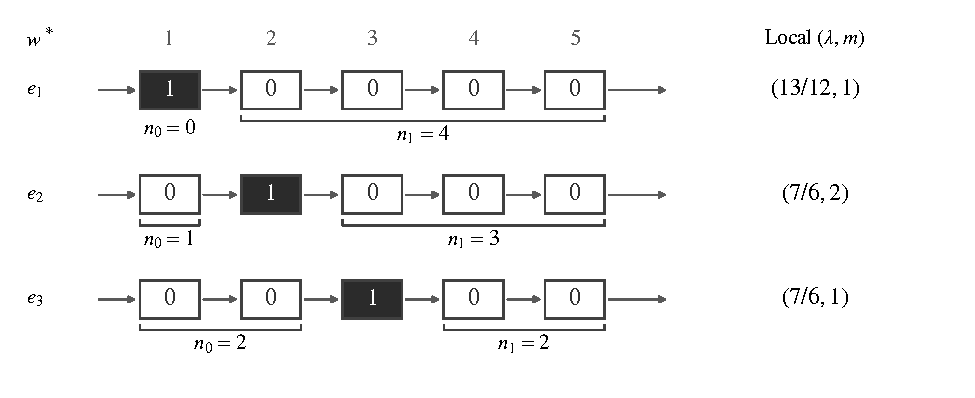
\includegraphics[width=\linewidth]{figures/active-arrangements.pdf}
\caption{The three distinct local pairs for the depth-five cubic target $f(x)=x+x^3$. Boxes denote full residual blocks, labeled by raw weight; black boxes are active, and brackets mark consecutive inactive groups. The endpoint, one-position-inward, and center placements have group lengths $(0,4)$, $(1,3)$, and $(2,2)$, respectively. Only the second has a group at the critical length $r=3$, giving $m=2$. By \eqref{eq:arrangementpair}, positions $5$ and $4$ have the same pairs as $1$ and $2$; see Table~\ref{tab:examples}.}\label{fig:arrangements}
\end{figure}

\begin{table}[H]
\centering
\begin{tabular}{@{}cccl@{}}
\toprule
Depth $L$ & Active position $j$ & Inactive lengths $(n_0,n_1)$ & Local $(\lambda,m)$\\
\midrule
4 & $1,4$ & $(0,3),(3,0)$ & $(1,2)$\\
4 & $2,3$ & $(1,2),(2,1)$ & $(1,1)$\\
5 & $1,5$ & $(0,4),(4,0)$ & $(13/12,1)$\\
5 & $2,4$ & $(1,3),(3,1)$ & $(7/6,2)$\\
5 & $3$ & $(2,2)$ & $(7/6,1)$\\
\bottomrule
\end{tabular}
\caption{The same cubic target at every listed realization. Positions are counted in composition order.}\label{tab:examples}
\end{table}
At depth four, moving the active block changes the logarithmic factor. At depth five, it can change the exponent itself. All these points have raw coefficient-Jacobian rank one; that rank does not determine either pair. The theorem also permits more than one logarithm: two groups of length $r$ give $m=3$. The global integral, however, depends on which of these local contributions dominates across the whole fiber.

\paragraph{Remark (what a local learning coefficient sees).}
Let $\varpi=\chi\pi\,dw$ be the local measure of \eqref{eq:pair}. Write $\mathcal Z(t)=\int e^{-tK_f}\,d\varpi$ and $E_t[K_f]=\mathcal Z(t)^{-1}\int K_fe^{-tK_f}\,d\varpi$; here $t$ plays the role of $n\beta$ for a tempered posterior. $K_f$ is bounded on the compact support, so differentiating under the integral gives $(\log\mathcal Z)'=-E_t[K_f]$. Integrating this and applying \eqref{eq:pair}, for each fixed $t_0>0$, with an $O(1)$ term depending on $t_0$, $w^*$ and $\mu$,
\begin{equation}\label{eq:llcaverage}
 \int_{t_0}^{T}E_t[K_f]\,dt=\lambda\log T-(m-1)\log\log T+O(1),\qquad T\to\infty.
\end{equation}
Dividing by $\log T$ shows that the average of $tE_t[K_f]$ against $dt/t$ tends to $\lambda$; the multiplicity enters only at the $\log\log T$ scale. At depth five the endpoint and center placements differ by $1/12$ in $\lambda$, while positions $2$ and $3$ share $\lambda=7/6$ and differ by $-\log\log T+O(1)$; at depth four all placements share $\lambda=1$. The limit therefore recovers $\lambda$ but not $m$, and only asymptotically. For position $2$, with $(7/6,2)$, against position $1$, with $(13/12,1)$, even after discarding the unknown $O(1)$ term, the displayed asymptotic terms have the expected ordering only for $\log T>46$. (The pointwise limit $tE_t[K_f]\to\lambda$ needs finer asymptotics than \eqref{eq:pair}.)

\section{Full fibers and global selection}
To determine the global pair, we compare the local contributions from every realization in the target fiber.
\begin{theorem}[Full fibers and global selection]\label{thm:global}\leantag{UnifiedNetworkCertificate}{53}
Assume \eqref{eq:gram} and $0\le k\le L$. Let $f=F_{c_k}\circ\cdots\circ F_{c_1}$, with $c_j\ne0$ and, for even $r$, $c_j>0$. For $k=0$, set $f=x$. In effective coordinates $u=w^r$, the complete fiber consists of the ordered coefficients $c_1,\ldots,c_k$ placed in any $k$ positions, with all other coefficients zero; the corresponding raw weights are $c_j^{1/r}$ for odd $r$ and $\pm c_j^{1/r}$ for even $r$. Its raw fiber $\mathcal F_f=\{w:K_f(w)=0\}$ has size
\[
 \#\mathcal F_f=\begin{cases}\binom Lk,&r\text{ odd},\\2^k\binom Lk,&r\text{ even}.\end{cases}
\]
For every prior satisfying the global conditions of Section~\ref{sec:model},
\begin{equation}\label{eq:globalpair}
 \int_{\R^L}e^{-N K_f(w)}\pi(w)\,dw
 \asym N^{-[k/2+A_r(L-k)]}(\log N)^{M_r(L-k)-1}.
\end{equation}
Repeated coefficients are allowed.
\end{theorem}


The ordered active coefficients can be recovered from the outermost active block inward. For normalized polynomials $H,G$ with constant coefficient zero and linear coefficient one, equality $H+cH^r=G+dG^r$ with $c,d\ne0$ forces $H=G$ and $c=d$. A leading-coefficient and degree argument proves this recovery step (Appendix~\ref{app:global}).

The identity loss is coercive, and the $L^2(\mu)$ triangle inequality gives
\[
 \sqrt{K_f(w)}\ge\sqrt{K_0(w)}-\norm{f-x}_{L^2(\mu)}.
\]
Thus $K_f$ has a positive gap outside small neighborhoods of its finite fiber, making the complementary integral exponentially small. Among local contributions, minimize $\lambda$, then maximize $m$ among ties. For $n=L-k$, the inequality $\sum_g\pos{n_g-r}\le\pos{n-r}$ gives \eqref{eq:globalpair} (Appendix~\ref{app:global}). The cubic examples have global pairs $(1,2)$ and $(13/12,1)$; a prior positive near another realization and supported in a sufficiently small neighborhood of it instead retains its local pair.

\section{Formal verification}\label{sec:formal}
Lean~4 certifies the pairs, fiber descriptions and counts of Theorems~\ref{thm:identity}--\ref{thm:global} for localizations on small balls with bounded measurable densities. The formalization also covers the inverse-power integrability criteria and the divergence at the endpoint, and the margin marks link each theorem to its certificate. The transfer to the smooth cutoffs of \eqref{eq:pair}, the zeta-pole interpretation and the two remarks are proved on paper or cited; meromorphic continuation and leading constants are not certified. Appendix~\ref{app:repro} records the snapshot, the principal declarations and the audit.


\section{Further directions}
A first extension concerns width-two cubic networks at depth four with one active block \citep{faber2026vector}. There an invertible active block has pair $(4,1)$ at every position, while a rank-one shear has $(4,5)$ in the first position and $(4,1)$ elsewhere: placement changes the multiplicity but not the exponent. Cancellation is governed by a binary cubic in each output row rather than by a sum of signed powers, which suggests a geometric version of the mechanism of Section~4. Biases add a translation symmetry in the setting of \citet{dahlgren2026}, and we have not studied its interaction with inactive groups. It is also open whether the transition at group length $r$ survives a lower-order term in the activation. Beyond plain residual blocks, the architectures we are studying now are blocks with separate read and write matrices, and networks without skip connections. Finally, these exact local pairs are targets for the estimator of \citet{lau2025}, and identifying which realization gradient-based training approaches would connect the calculation to practice. We kept the haystacks tiny so that each one could be searched to the bottom. The larger ones are next, and in the first of them the needle already hides differently.

\clearpage
\appendix
\section{Coefficient reduction, zeros, and coercivity}\label{app:coeff}
Write $h_\ell=xT_\ell(x^{r-1})$. The exact recursion
\[
 T_0(y)=1,\qquad T_\ell(y)=T_{\ell-1}(y)+u_\ell yT_{\ell-1}(y)^r
\]
shows that $h_L-x=\sum_{j=1}^{\nu} P_j(u)x^{d_j}$, where $P_j$ is homogeneous of degree $j$. Comparing the first two coefficients gives $P_1=S$ and $P_2=B=r(S^2-Q)/2$. At depth one there is no second coefficient, and $B=0$ because $Q=S^2$.

In a fixed small ball in effective variables, $|P_j(u)|\le C_j\norm{u}^j\le C_jQ$ for $j\ge2$. Hence the Gram upper bound gives $K_0\le C(S^2+Q^2)$. Conversely, with $\gamma>0$ the smallest eigenvalue of $G$,
\begin{equation}\label{eq:coercive}
 K_0\ge\gamma(S^2+B^2),\qquad
 Q=S^2-2B/r\le S^2+2|B|/r.
\end{equation}
Locally $S^4\le C S^2$, so $Q^2\le C(S^2+B^2)$. This proves \eqref{eq:identityreduction}. Globally \eqref{eq:coercive} gives
\[
 Q\le K_0/\gamma+(2/r)\sqrt{K_0/\gamma}.
\]
Since $Q=\sum_iw_i^{2r}\to\infty$ as $\norm{w}\to\infty$, $K_0$ is coercive. Also $K_0=0$ implies $S=B=Q=0$, hence $w=0$. For a finite-mass prior the integral outside any sufficiently small fixed neighborhood is therefore $O(e^{-bN})$ for some $b>0$.

\section{Angular sectors and the logarithmic factor}\label{app:sectors}
For even $r$, $S\asym\norm{w}^r$ and \eqref{eq:identityreduction} reduces the integral to an ordinary radial integral with density $\rho^{L-1}$ and loss $\rho^{2r}$. The pair is $(L/(2r),1)$. At depth one the loss is exactly a positive constant times $w^{2r}$ for either parity.

Suppose $r$ is odd and $L\ge2$, and use the Euclidean sphere. Let $\tau(\theta)=\sum_i\theta_i^r$, $q(\theta)=\sum_i\theta_i^{2r}$. Compactness gives $0<c\le q\le C$. The set $\Sigma=\{\tau=0\}$ is nonempty, since it contains $(2^{-1/2},-2^{-1/2},0,\ldots,0)$. At a point of $\Sigma$, Euler's identity gives $\theta\cdot\nabla\tau=r\tau=0$, whereas $\nabla\tau\ne0$. Thus the tangential derivative is nonzero. The inverse function theorem supplies smooth local coordinates $(t,\eta)$ with $t=\tau$, and surface density bounded above and below on smaller coordinate boxes. A finite collection of these boxes covers a neighborhood of the compact set $\Sigma$. On the remaining compact angular set, $|\tau|$ has a positive lower bound.

Restrict each chart to the inverse image of a product box $|t|<b$, $\eta\in V$ contained in its image; finitely many smaller boxes cover $\Sigma$, and bounded larger boxes give upper bounds. The smaller boxes give lower bounds, while the unused coordinates contribute finite positive volume. For radial cutoff $R>0$, the product domain lies between $(0,\rho_0)\times(-\rho_0^r,\rho_0^r)$ and $(0,\rho_1)\times(-\rho_1^r,\rho_1^r)$, where $\rho_0=\min(R,b^{1/r})$ and $\rho_1=\max(R,b^{1/r})$. These inclusions let us bound the integral by the same model expression on smaller and larger boxes. The comparison \eqref{eq:angularmodel} is used only on the chart domain itself; the larger boxes carry only the explicit model integrand, so they give valid upper bounds.

The reduced loss equals $\rho^{2r}(t^2+\rho^{2r}q^2)$ and is comparable to \eqref{eq:angularmodel}. In a product box $0<\rho<\rho_0$, $|t|<\rho_0^r$, split into two sectors for each sign $\sigma\in\{-1,1\}$:
\begin{align*}
 \mathcal C:&\quad t=\sigma\rho^r v,\quad 0<v<1,
 &&\rho^{L-1}d\rho\,dt=\rho^{L+r-1}d\rho\,dv,\\
 \mathcal O:&\quad t=\sigma z^r,\quad \rho=zy,
 &&\rho^{L-1}|d\rho\,dt|=r z^{L+r-1}y^{L-1}dz\,dy,\\
 &\quad 0<z<\rho_0,\ 0<y<1.
\end{align*}
Apart from boundaries of measure zero these are exactly $|t|<\rho^r$ and $\rho^r<|t|$. The loss is comparable to $\rho^{4r}$ in $\mathcal C$ and to $z^{4r}y^{2r}$ in $\mathcal O$. Sector $\mathcal C$ has pair $((L+r)/(4r),1)$. For $\mathcal O$, substitute $a=z^{4r}$ and $b=y^{2r}$. Up to constants its integral is
\[
 \int_0^{\rho_0^{4r}}\!\int_0^1 e^{-Nab}a^{\alpha-1}b^{\beta-1}\,db\,da,
 \qquad \alpha=\frac{L+r}{4r},\quad\beta=\frac{L}{2r}.
\]
The inner integral is comparable to $\min\{1,(Na)^{-\beta}\}$. Splitting at $a=N^{-1}$ gives order $N^{-\min(\alpha,\beta)}$, with a factor $\log N$ exactly when $\alpha=\beta$. The same pair follows directly from the integer monomial $z^{4r}y^{2r}$ with density $z^{L+r-1}y^{L-1}$ by \citet[Proposition 2.1]{lin2017}. The noncancellation region contributes $O(N^{-\beta})$, so it does not change the resulting pair. The same integrals with the exponential replaced by the negative power diverge when either exponent reaches its critical value.

Finally, if $cF\le K\le CF$, then the corresponding Laplace integrals satisfy $Z_F(CN)\le Z_K(N)\le Z_F(cN)$ for the same positive amplitude. Thus both the exponent and the logarithmic power transfer to the actual loss. For the pole interpretation, replace the cutoff by a small closed box around the isolated zero, on which the density is smooth and positive. The difference is supported away from the zero and contributes an exponentially small Laplace term and a zeta term holomorphic near the positive real axis. Resolution on that box supplies the stated interpretation.

The Lean certificates localize to balls rather than smooth cutoffs. If $B_{\rm in}\subset\{\chi=1\}$ and $\supp\chi\subset B_{\rm out}$ are small balls around $w^*$, then
\[
 \int_{B_{\rm in}}e^{-NK_f}\pi\,dw\le Z_{N,w^*}\le\norm{\chi}_\infty\int_{B_{\rm out}}e^{-NK_f}\pi\,dw.
\]
Both outer integrals have the same pair, since any sufficiently small ball does, so $Z_{N,w^*}$ has it too.

For the integrability threshold, Tonelli and $\int_0^\infty t^{s-1}e^{-tK}\,dt=\Gamma(s)K^{-s}$ give, for $s>0$,
\[
 \int K_f^{-s}\chi\pi\,dw=\frac1{\Gamma(s)}\int_0^\infty t^{s-1}Z_{t,w^*}\,dt,
\]
because the zero set of $K_f$ meets a small $\supp\chi$ only in the null set $\{w^*\}$. Near $t=0$ the integrand is integrable for every $s>0$; at infinity \eqref{eq:pair} makes it integrable exactly when $s<\lambda$. For $s\le0$ integrability is trivial.

\section{Proof of the local arrangement theorem}\label{app:arrangement}
The proof isolates independent leading directions in coefficient space and bounds the higher-order terms relative to them, even along cancellation paths. The Gram assumption then transfers the resulting coefficient comparison to the population loss, after which the local integral factors.

Fix $r,k,(n_g)$ and nonzero active coefficients $c_1,\ldots,c_k$. Constants in the coefficient estimates, and the size of the neighborhood, depend only on these fixed data; they may degenerate as some $c_j\to0$. Use coefficient $\ell^1$ norms on polynomial spaces and sum norms on their direct sums; use the Euclidean norm on each effective group vector $u_g=(a_{g,i}^r)_i$. Norm equivalence will be used only in fixed finite dimension.

\paragraph{The auxiliary composition map.}
Set $d_h=1+h(r-1)$, $\nu_g=(r^{n_g}-1)/(r-1)$, and
\[
 \mathcal P_g=\operatorname{span}\{x^{d_h}:1\le h\le\nu_g\},\qquad
 \mathcal P=\R^k\oplus\bigoplus_{g=0}^k\mathcal P_g.
\]
Thus $\mathcal P_g=\{0\}$ for an empty group and $\mathcal P_g=\operatorname{span}\{x^r\}$ for a singleton. For $v=(\delta,p_0,\ldots,p_k)\in\mathcal P$, define
\begin{equation}\label{eq:Psi}
 \Psi(v)=(\operatorname{id}+p_k)\circ F_{c_k+\delta_k}\circ\cdots
 \circ(\operatorname{id}+p_1)\circ F_{c_1+\delta_1}\circ(\operatorname{id}+p_0).
\end{equation}
For $k=0$ this means $\Psi(p_0)=\operatorname{id}+p_0$. This is a polynomial map into the finite-dimensional space of polynomials of degree at most $r^L$: degrees multiply, and $k+\sum_g n_g=L$. Every output has linear term $x$, and its other degrees are $1$ modulo $r-1$, so all output differences lie in the sparse feature space of \eqref{eq:gram}. Let $\mathcal H_g$ denote the composition of inactive group $g$. For its error $p_g=\mathcal H_g-x$, $\Psi(v)=h_L$ and $\Psi(0)=f$.

The differential can be identified exactly. Put $\widehat H_0=x$, $\widehat H_j=F_{c_j}\circ \widehat H_{j-1}$, and $T_j=F_{c_k}\circ\cdots\circ F_{c_{j+1}}$, with $T_k=\operatorname{id}$. Define the fixed polynomials
\[
 U_j=(T_j'\circ \widehat H_j)\widehat H_{j-1}^r,\quad
 V_g=(T_g'\circ \widehat H_g)\widehat H_g^r,\quad
 W_g=(T_g'\circ \widehat H_g)\widehat H_g^{2r-1}.
\]
The chain rule gives, for arbitrary auxiliary group perturbations $q_g\in\mathcal P_g$,
\begin{equation}\label{eq:dPsi}
 D\Psi(0)[\alpha,q_0,\ldots,q_k]
 =\sum_{j=1}^k\alpha_j U_j+\sum_{g=0}^k(T_g'\circ \widehat H_g)(q_g\circ \widehat H_g).
\end{equation}
In particular $V_g$ and $W_g$ are the columns for the first two group coefficients when those coefficients exist.

\paragraph{Independence for $r\ge3$.}
First consider the virtual family $U_j,V_g,W_g$ in $\R[x]$, including both directions at every group. At $k=0$ the family is $x^r,x^{2r-1}$. Suppose the family at $j$ active blocks is independent and has degrees at most $(2r-1)d$, where $d=r^j$ is the degree of the partial output $H$. Appending $F_e$, $e\ne0$, multiplies all old columns by $P=1+reH^{r-1}$ and adds the active column $H^r$ and the last-group columns $\widetilde H^r,\widetilde H^{2r-1}$, where $\widetilde H=H+eH^r$.

The multiplied old degrees are at most $(3r-2)d$; the last two degrees are $r^2d$ and $r(2r-1)d$, strictly greater and distinct for $r\ge3$. Their coefficients in any relation therefore vanish. The remaining relation is $PR+tH^r=0$. Since $P-reH^{r-1}=1$, $P$ and $H^r$ are coprime. The polynomial $P$ is nonconstant, so $P\mid tH^r$ forces $t=0$, then $R=0$. This proves independence and preserves the degree bound. Delete both group columns for an empty group and $W_g$ for a singleton. The remaining columns are independent and, by \eqref{eq:dPsi}, belong to the actual sparse output space. The virtual columns need not belong to that space and are used only to prove independence before restriction.

\paragraph{Uniform control of omitted coefficients.}
Each actual inactive group has
\begin{equation}\label{eq:group}
\begin{gathered}
 \mathcal H_g=x+S_gx^r+B_gx^{2r-1}+R_g,\\
 B_g=\frac r2(S_g^2-Q_g),\qquad
 \norm{R_g}\le C_g\norm{u_g}_2Q_g.
\end{gathered}
\end{equation}
Indeed its coefficient of $x^{d_h}$ is homogeneous of degree $h$ in $u_g$. On $\norm{u_g}_2\le1$, the sum of the finitely many terms with $h\ge3$ is bounded by $C_g\norm{u_g}_2^3$, and $Q_g=\norm{u_g}_2^2$. Empty and singleton groups have $R_g=0$; also $B_g=0$ for a singleton.

For odd $r$, let $z$ consist of the active deviations, $S_g$ for $n_g\ge1$, and $B_g$ for $n_g\ge2$. Let $J$ insert these scalars as the corresponding auxiliary coordinates; its norm is one. With
\[
 \varepsilon=\sum_j|\delta_j|+\sum_g\norm{u_g}_2,\qquad
 R=(0,R_0,\ldots,R_k),
\]
we have the \emph{exact identity} $v=Jz+R$. Shrink the neighborhood so $\varepsilon\le1$ and $|S_g|\le1$ for every group. Since
\[
 Q_g\le S_g^2+\frac2r|B_g|\le |S_g|+\frac2r|B_g|,
\]
\eqref{eq:group} gives fixed constants $C_0,C_1>0$ such that
\begin{equation}\label{eq:zcontrol}
 \norm{z}\le C_0\varepsilon,\qquad \norm{R}\le C_1\varepsilon\norm{z}.
\end{equation}
The first bound follows from $|S_g|\le\sqrt{n_g}\norm{u_g}_2$ and $|B_g|\le C\norm{u_g}_2^2$. No division by $S_g$, $B_g$ or $\norm{z}$ occurs, so the bounds hold through simultaneous cancellations, including $z=0$.

\begin{lemma}[Taylor estimate with a controlled remainder]\label{lem:remainder}
Let $\Psi$ be a $C^2$ map between finite-dimensional normed spaces on a neighborhood of the closed unit ball. Let $J$ be linear and suppose $v=Jz+R$, $0\le\varepsilon\le1$, and \eqref{eq:zcontrol} holds. Set $M=\norm{J}+C_1$, and assume $MC_0\varepsilon\le1$. If $H_*$ bounds $\norm{D^2\Psi}$ on that ball, then, with $A=D\Psi(0)J$,
\begin{equation}\label{eq:explicitE}
 \Psi(v)-\Psi(0)=Az+E,\qquad
 \norm{E}\le\left(\norm{D\Psi(0)}C_1+\frac {H_*}2 M^2C_0\right)\varepsilon\norm{z}.
\end{equation}
\end{lemma}
\begin{proof}
We have $\norm{v}\le M\norm{z}\le MC_0\varepsilon\le1$. Taylor's formula with its integral remainder gives the exact decomposition
\[
 E=D\Psi(0)R+\int_0^1(1-t)D^2\Psi(tv)[v,v]\,dt.
\]
The first term is bounded by $\norm{D\Psi(0)}C_1\varepsilon\norm{z}$. The second is bounded by
\[
 (H_*/2)\norm{v}^2\le(H_*/2)M^2\norm{z}^2\le(H_*/2)M^2C_0\varepsilon\norm{z}.
\]
\end{proof}

Apply the lemma to \eqref{eq:Psi}; a finite $H_*$ exists by compactness because $\Psi$ is polynomial. The retained-column independence gives $a>0$ with $\norm{Az}\ge a\norm{z}$. Let $C_*$ be the parenthesized constant in \eqref{eq:explicitE}. Choose $\varepsilon$ small enough that $MC_0\varepsilon\le1$ and $C_*\varepsilon\le a/2$, in addition to the preceding group bounds. Then
\[
 \frac a2\norm{z}\le\norm{h_L-f}\le(\norm{A}+a/2)\norm{z}.
\]
All these restrictions hold on a full neighborhood of the fixed raw realization because $\varepsilon\to0$ there. Norm equivalence, \eqref{eq:group}, and the sparse Gram bounds give
\[
 K_f\asym\sum_j\delta_j^2+\sum_g(S_g^2+B_g^2)
 \asym\sum_j\delta_j^2+\sum_g(S_g^2+Q_g^2).
\]
For the last comparison use $Q_g\le S_g^2+2|B_g|/r$ and $B_g=r(S_g^2-Q_g)/2$ with bounded $S_g$.

\paragraph{Even degree, including $r=2$.}
Now $u_g\ge0$, so $Q_g\le S_g^2$. Retain $z=(\delta,S_g:n_g\ge1)$ and set $R'_g=\mathcal H_g-x-S_gx^r$. Homogeneity of all omitted coefficients, now of degree at least two, gives
\[
 \norm{R'_g}\le C_g Q_g\le C_g S_g^2
 \le C_g\sqrt{n_g}\,\varepsilon S_g.
\]
Thus $v=Jz+(0,R'_0,\ldots,R'_k)$ obeys the same lemma. The retained family $U_j,V_g$ is independent by the previous induction with old degree bound $rd$, multiplied bound $(2r-1)d$, and new last-group degree $r^2d>(2r-1)d$ for every $r\ge2$; coprimality separates the new active column. Absorption yields $K_f\asym\sum_j\delta_j^2+\sum_g S_g^2$. Finally
\[
 \sum_{i\text{ in }g}|w_i|^{2r}\le S_g^2
 \le n_g\sum_{i\text{ in }g}|w_i|^{2r}
\]
for each nonempty group, proving \eqref{eq:arrangementeven}.

\paragraph{Integration.}
The Jacobian determinant of the active coordinate map is $\prod_j r(w^*_{i_j})^{r-1}\ne0$. Its inverse absolute Jacobian and the prior are bounded above and away from zero locally. Inner and outer product boxes in $(\delta,a_0,\ldots,a_k)$ bound the cutoff integral. On each box the comparison integral factors into Gaussian active integrals and identity-group integrals. Theorem~\ref{thm:identity}, or the usual addition rule \citep[Proposition 3.7]{lin2017}, gives \eqref{eq:arrangementpair}: exponents add and $m-1=\sum_g(M_r(n_g)-1)$. All comparison losses vanish only at the base point, so shrinking cutoffs does not change the pair.

\section{Full fibers and global selection}\label{app:global}
\paragraph{Ordered recovery.}
Every active block has degree $r$, so a network with $q$ active blocks has degree $r^q$. Equal outputs therefore have the same active count. To recover their coefficients, suppose
\[
 H+cH^r=G+dG^r,\qquad c,d\ne0,
\]
where $H(0)=G(0)=0$ and $H'(0)=G'(0)=1$. Equality of output degrees gives $\deg H=\deg G=D\ge1$. Choose $a\ne0$ so that $U=aG$ and $H$ have the same leading coefficient. Comparing leading output coefficients gives $d=ca^r$, hence
\[
 c(H-U)\sum_{i=0}^{r-1}H^iU^{r-1-i}=G-H.
\]
The sum has degree $(r-1)D$: its leading coefficient is $r$ times the $(r-1)$st power of the common leading coefficient. If $H-U\ne0$, its zero constant coefficient forces degree at least one. The left side would then have degree greater than $D$, while the right side has degree at most $D$. Thus $H=U$; the linear coefficients give $a=1$, and consequently $H=G$ and $c=d$. Iterating this step recovers the ordered active chain.

\paragraph{Fiber size.}
The positive-definite feature Gram makes zero population loss equivalent to polynomial equality. The recovered chain can occupy any $k$ of the $L$ positions, in its fixed order. Each placement has one raw realization for odd $r$ and $2^k$ independent sign choices for even $r$. Different supports or signs give different vectors, even when active coefficients repeat. This proves the stated count.

\paragraph{Global selection.}
Coercivity from Appendix~\ref{app:coeff} and the $L^2$ triangle inequality make every sublevel set of $K_f$ compact. Remove disjoint small neighborhoods of the finite fiber from the integration domain. Choose a large ball outside which $K_f\ge1$. Within the ball, the complement of the open fiber neighborhoods is compact and zero-free, so continuity gives a positive minimum whenever that complement is nonempty. Set $b=1$ if that complement is empty; otherwise take the smaller of its minimum and one. Then $K_f\ge b>0$ on the entire remaining set, so the prior-weighted tail is at most $e^{-bN}\int\pi$. Continuity and positivity of the prior at each fiber point give local upper and positive lower bounds. Each fiber neighborhood therefore has the pair of Theorem~\ref{thm:arrangement} with a positive contribution. A finite sum of terms $N^{-\lambda_i}(\log N)^{m_i-1}$ has the smallest $\lambda_i$ and then the largest $m_i$ among ties. Several realizations with that same pair affect the multiplicative constants, not the logarithmic power; multiplicities do not add across disjoint neighborhoods.

For even $r$, every placement has pair $(k/2+(L-k)/(2r),1)$. For odd $r$, write $n=L-k=\sum_g n_g$. Then
\[
 \sum_g A_r(n_g)=\frac n{2r}-\frac1{4r}\sum_g\pos{n_g-r},\qquad
 \sum_g\pos{n_g-r}\le\pos{n-r}.
\]
If $n<r$, all placements have the same exponent and $m=1$. If $n=r$, all exponents agree and concentrating the inactive blocks in one gap gives $m=2$, the largest multiplicity. If $n>r$, the inequality is strict whenever at least two gaps are nonempty: if any gap exceeds $r$, the other nonempty gaps strictly reduce the sum of positive parts from $n-r$; if none does, that sum is zero. Hence concentration in one gap uniquely describes the minimizing patterns, and these have $m=1$. Such a placement exists before, between, or after the ordered active blocks. This proves \eqref{eq:globalpair}.

\section{Lean source and audit record}\label{app:repro}
The proof source is available at
\begin{center}\small\url{https://github.com/bubskee/residual-slt-in-a-haystack}\end{center}
The reproducibility snapshot, containing the proof source and audit, is
\begin{center}\small\ttfamily b08b1a334abac97cbdf754ba14eacee82e10be70\end{center}
It uses Lean \texttt{v4.35.0} and mathlib commit
\begin{center}\small\ttfamily 56a005855ea17e0b0958f73ec801ae140b0a1679\end{center}
The principal declarations, all in namespace \texttt{ResidualSLT}, are
\begin{itemize}\setlength{\itemsep}{0pt}
\item \leanname{unified_residual_network_certificate}: full fibers, exact counts, and local/global learning pairs;
\item \leanname{sparse_identity_network_rlct_laplace_certificate}: the identity pair;
\item \leanname{arrangement_raw_network_rlct_laplace_certificate_of_depth_pos}: the local arrangement pair;
\item \leanname{network_full_raw_fiber}: ordered active-chain classification;
\item \leanname{raw_network_fiber_cardinality}: exact raw-fiber size.
\end{itemize}

\noindent\begin{minipage}{\linewidth}
Exact hypotheses are recorded in \path{paper/formalization_status.md}. From the repository root, run:
\begingroup\small
\begin{verbatim}
git checkout b08b1a334abac97cbdf754ba14eacee82e10be70
cd lean
lake exe cache get
lake build
lake env lean -DwarningAsError=true -DautoImplicit=false \
  ../paper/checks/NetworkAudit.lean
\end{verbatim}
\endgroup
\end{minipage}

The audit prints the certificate definitions and the types and axiom dependencies of these five declarations. Every dependency set is exactly \texttt{propext}, \texttt{Classical.choice}, and \texttt{Quot.sound}; none contains \texttt{sorryAx}. The logs are in \path{paper/checks/}: \mbox{\path{lean-build.txt}} and \mbox{\path{NetworkAudit.txt}}.

\paragraph{Tool and computational resource disclosure.}
Following the disclosure recommendation of the Leiden Declaration on Artificial Intelligence and Mathematics \citep{leiden2026}, we report substantial AI assistance. Astra and Opus 5.5 assisted with writing, proof development, and Lean formalization. Fable 5.1 provided adversarial review and attempted to find errors in the arguments. The author retains responsibility for the results, arguments, and citations.

\paragraph{Acknowledgments.}
The author thanks the early readers in the Mechanistic Interpretability Discord for their comments on a draft, and BlueDot Impact for financial support.

\bibliographystyle{plainnat}
\begingroup\small
\setlength{\bibsep}{4pt}
\bibliography{references}
\endgroup
\end{document}
